\documentclass[conference,onecolumn,a4paper,romanappendices,12pt,english,nofonttune]{IEEEtran}
\IEEEoverridecommandlockouts

\usepackage{cite}
\usepackage{amsmath,amssymb,amsfonts}
\usepackage{algorithmic}
\usepackage{graphicx}
\usepackage{textcomp}
\usepackage{xcolor}
\def\BibTeX{{\rm B\kern-.05em{\sc i\kern-.025em b}\kern-.08em
    T\kern-.1667em\lower.7ex\hbox{E}\kern-.125emX}}

    
\begin{document}

\title{Your Digest Title*}

% \thanks{Identify applicable funding agency here. If none, delete this.}

\vspace{30pt}
\author{\IEEEauthorblockN{\color{red} THIS IS A BLIND REVIEW. DO NOT INCLUDE AUTHOR INFORMATION!!!}
}
\vspace{30pt}

\maketitle

\begin{abstract}
Type your abstract here.  We prefer an abstract that is between 100 and 200 words.  IMPORTANT: no author names or affiliations are to be listed.  
\end{abstract}

\begin{IEEEkeywords}
component, formatting, style, styling, insert
\end{IEEEkeywords}

\section{INTRODUCTION}
The digest is meant to be a short version of your intended paper that facilitates quick and easy review. The main body of your digest, starting with the \textbf{ABSTRACT} and ending with the \textbf{CONCLUSIONS}, must be less than five pages long. Use at least 11 pt font (12 pt is preferred), double-spacing, and 2.5 cm margins.

Note that reducing line spacing \textbf{OR} using excessively dense formatting to include more content is not appropriate for a fair review process. Any digest that exceeds \textbf{2500 words} (excluding the \textbf{REFERENCES} section) may be rejected and excluded from the technical review process.

You are required to submit references as part of the digest. The \textbf{REFERENCES} section should start on a standalone page, and it is not included in the five-page limit. The references section can be as long as you need, can be single-line spaced, and may put the total digest over the five-page limit.

Please bear in mind that conference reviewers often have to review many digests, so \textbf{please do not submit a full-length, single-spaced paper that is simply cropped down to five pages}.


\section{FIRST SECTION}
Enter text, equations, and figures for your first full section here. You do not need to follow this format exactly, but it is suggested by the Program Committee. See Fig.~\ref{fig:sample} for a sample figure.

\begin{figure}[h!]
    \centering
    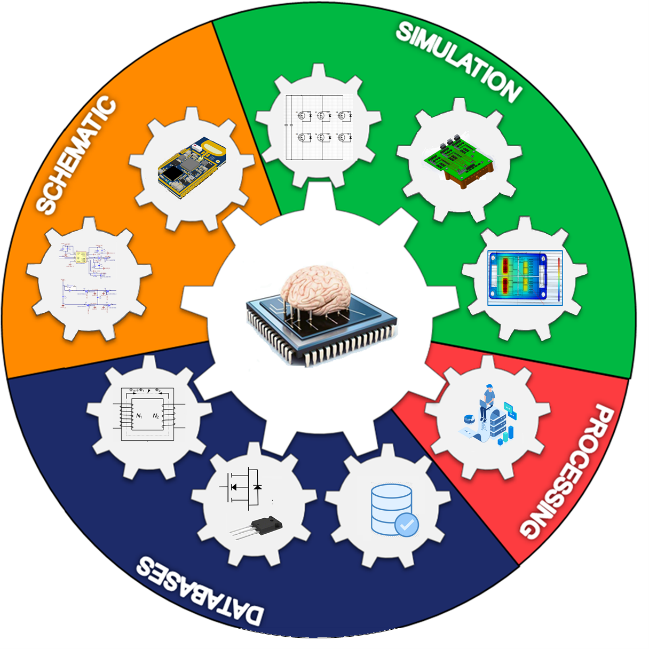
\includegraphics[width=6cm]{sample_figure.png} % Replace with your figure file
    \caption{Sample figure.}
    \label{fig:sample}
\end{figure}

\section{SECOND SECTION}
Enter text, equations, and figures for your second full section here. Repeat as necessary for other sections. Equations should be expressed in the following format:

\begin{equation}
    A = \pi r^2
\end{equation}

\section{CONCLUSIONS AND FUTURE WORK}
State your conclusions here and your plans for the final submission of a full paper, assuming your digest is accepted. Please clearly state your contributions compared with previous works, and list relevant references in the following \textbf{REFERENCES} section.

You are reminded that the reviewers will prize experimental results and real-world applications, and as such, you should be sure to address these points in your digest. Evidence of completed experimental work will naturally be prized more than promises of future experimental work.

\textbf{IMPORTANT:} This section is the last section in your five-page limit. If you let content bleed onto the sixth page, your submission will be automatically \textbf{REJECTED}.

\newpage
{\color{red}Note: references are required. This section should start on a separate page and it is not included in the five-page limit.  References can be single-spaced.References to articles can be made using \verb|\cite{b1,b2,b3}| e.g. \cite{b1,b2,b3}.}
\bibliographystyle{IEEEtran}
\bibliography{References}

\vspace{30pt}
{\color{red}Alternatively, the incorporation of input references may be executed as follows:}

\begin{thebibliography}{00}

\bibitem{b1} J. Doe, J.F. Stevens, and B. Smith, ``Title of their journal paper,'' \textit{Journal Title}, vol. 17, no. 1, pp. 123--133, Feb. 2005.
\bibitem{b2} N. Surname and N. Surname, ``Title of their conference paper,'' in \textit{IEEE 1997 Conference Name}, 2017, pp. 122--129.
\bibitem{b3} A.C. Doyle, \textit{Title of book}, Publisher’s Name, City, 2020.
\end{thebibliography}
\vspace{12pt}
\end{document}
